% file: rapport.tex
% date: 04/12/2020
% author: Benjamin PONTON bponton@enseirb-matmeca.fr
%         Enzo MEDINA emedina@enseirb-matmeca.fr


\documentclass[a4paper]{article}

\usepackage[utf8]{inputenc}
\usepackage[french]{babel}
\usepackage{graphicx}
\graphicspath{{./graphic/}}
\usepackage{amsmath, amssymb}
\usepackage[left=3cm,right=3cm,top=2cm,bottom=2cm]{geometry}
\usepackage{url}
\usepackage[T1]{fontenc}
\usepackage{fullpage}
\usepackage{color}
\usepackage{listings}
\usepackage{algorithm}
\usepackage{algorithmic}


\definecolor{codegreen}{RGB}{32, 124, 47}
\definecolor{mygray}{RGB}{149, 152, 150}

\lstset{
  aboveskip=3mm,
  belowskip=-2mm,
  backgroundcolor=\color{white},
  basicstyle=\footnotesize,
  breakatwhitespace=false,
  breaklines=true,
  captionpos=b,
  commentstyle=\color{codegreen},
  deletekeywords={...},
  escapeinside={\%*}{*)},
  extendedchars=true,
  framexleftmargin=16pt,
  framextopmargin=3pt,
  framexbottommargin=6pt,
  frame=tb,
  keepspaces=true,
  keywordstyle=\color{blue},
  language=C,
  literate=
  {²}{{\textsuperscript{2}}}1
  {⁴}{{\textsuperscript{4}}}1
  {⁶}{{\textsuperscript{6}}}1
  {⁸}{{\textsuperscript{8}}}1
  {€}{{\euro{}}}1
  {é}{{\'e}}1
  {è}{{\`{e}}}1
  {ê}{{\^{e}}}1
  {ë}{{\¨{e}}}1
  {É}{{\'{E}}}1
  {Ê}{{\^{E}}}1
  {û}{{\^{u}}}1
  {ù}{{\`{u}}}1
  {â}{{\^{a}}}1
  {à}{{\`{a}}}1
  {á}{{\'{a}}}1
  {ã}{{\~{a}}}1
  {Á}{{\'{A}}}1
  {Â}{{\^{A}}}1
  {Ã}{{\~{A}}}1
  {ç}{{\c{c}}}1
  {Ç}{{\c{C}}}1
  {õ}{{\~{o}}}1
  {ó}{{\'{o}}}1
  {ô}{{\^{o}}}1
  {Õ}{{\~{O}}}1
  {Ó}{{\'{O}}}1
  {Ô}{{\^{O}}}1
  {î}{{\^{i}}}1
  {Î}{{\^{I}}}1
  {í}{{\'{i}}}1
  {Í}{{\~{Í}}}1,
  morekeywords={*,...},
  numbers=left,
  numbersep=10pt,
  numberstyle=\tiny\color{black},
  rulecolor=\color{black},
  showspaces=false,
  showstringspaces=false,
  showtabs=false,
  stepnumber=1,
  stringstyle=\color{black},
  tabsize=4,
  title=\lstname,
}




\begin{document}

\begin{titlepage}
    \begin{sffamily}
    \begin{center}
    
    ~\\[3cm]
    \textsc{\LARGE ENSEIRB-MATMECA}\\[1.5cm]
    
    \textsc{\Large Filière Informatique - 1ère année}\\[2cm]
    
    
        % Title
        \hrulefill \\[0.4cm]
    { \Huge \bfseries Rapport de projet \\[0.4cm] }
    { \huge \bfseries Tuiles de Wang \\[0.4cm] }
     \hrulefill \\[2cm]
     
     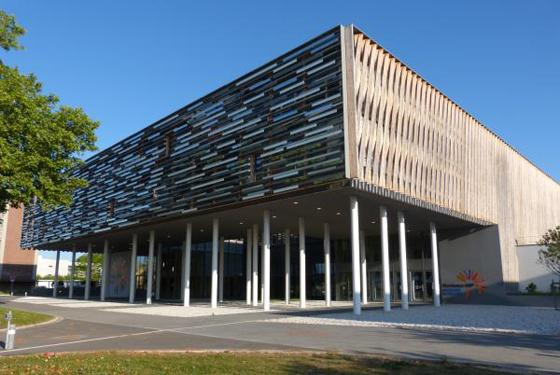
\includegraphics[scale=0.6]{enseirb_matmeca.jpg} \\[1cm]
     
    % Authors
    \begin{minipage}{0.4\textwidth}
      \begin{flushleft} \large
         \emph{Auteurs :} \\
        Enzo MEDINA\\
        Benjamin PONTON\\
      \end{flushleft}
    \end{minipage}
    \begin{minipage}{0.4\textwidth}
      \begin{flushright} \large
        \emph{Encadrants :} \\
        M. David RENAULT\\
        M. Jean-Luc BIENVENU\\
      \end{flushright}
    \end{minipage}
    \\[1cm]
    
    {\large 3 Novembre 2020 — 18 Décembre 2020}
    
    \end{center}
    \end{sffamily}
\end{titlepage}


\tableofcontents

\newpage

\section{Introduction}


\subsection{Objectif du projet}
Ce projet, sous forme d'un travail en binôme de 6 semaines, a pour objectif final la réalisation d'un jeu en langage de programmation C. Il vise à nous apprendre à travailler en groupe, à nous organiser, à rendre un travail dans les délais et à développer nos compétences techniques sur des sujets complexes, compétences requises pour un ingénieur. Le projet commence par une version initiale qui est ensuite améliorée à travers plusieurs 'achievements', qui seront expliqués au fur et à mesure dans ce rapport.

\subsection{Principe du jeu}
La version de base du jeu, Tilings, met en scène plusieurs joueurs qui s'affrontent sur un plateau de jeu. Ils possèdent tous un deck, composé de tuiles de Wang (carrés de 4 triangles colorés). Après que le premier joueur ait déposé une tuile au centre, les joueurs posent ensuite, à tour de rôle, la tuile au sommet de leur deck, en s'assurant que l'ensemble des tuiles soit connexe et que deux côtés de tuiles adjacents soient de même couleur. Si l'un des joueurs ne peut pas poser de tuile, il saute son tour et il range sa tuile au fond de son deck. La partie s'arrête, si lors d'un tour tous les joueurs ont sauté leur tour ou si l'un d'eux n'a plus de tuiles. Le décompte des points est calculé selon différentes méthodes au cours des achievements. Au début, le nombre de points est égal au nombre de tuiles posées.

\section{Cadre de travail}

\subsection{Répartition des tâches}
La répartition des tâches dans le binôme s'est faîte naturellement. Nous avons chacun choisi des fichiers pour éviter un maximum de conflits et donc gagner du temps. Enzo MEDINA s'est occupé en majorité de \fbox{color.c}, de \fbox{file.c} et de \fbox{project.c} et Benjamin PONTON de \fbox{tile.c} et de l'ensemble des tests en général (\fbox{test rule.c}, \fbox{test tile.c}, etc). Cependant, pour le fichier \fbox{rule.c}, qui contient la majorité des fonctions qui permettent le bon déroulement du jeu, nous avons travaillé ensemble.

\subsection{Organisation du travail}
Au niveau de l'organisation du travail, nous avions des séances le mardi et le vendredi de 13h50 à 18h10 avec nos encadrants. En travaillant durant ces horaires, nous avons alors pu dresser des comptes rendus pour chacune de ces séances afin d'organiser notre travail :

\begin{tabular}{|c|l|l|} \hline
     Séances & Compte Rendu & To do \\
     & & \\
     \hline
     
     Séance 03/11 
     %Compte rendu                          %To do
     & - Découverte des fichiers fournis & - Bien comprendre le sujet \\ 
     & - Découverte du sujet & \tabularnewline
     \hline
     
     Séance 06/11 
     %Compte rendu                          %To do
     & - Fichier color.c et couleur.c implémentés & - Mettre en place l'initialisation \tabularnewline
     \hline
     
     Séance 10/11 
     %Compte rendu                          %To do
     & - Création des files & - Terminer la boucle de jeu \\
     & - Début de la boucle de jeu & - Finir les règles du jeu \\
     & - Début des règles du jeu & \tabularnewline
     \hline
     
     Séance 13/11
     %Compte rendu                          %To do
     & - Fin de la boucle de jeu & - Tester le programme \\
     & - Implémentations des fonctions en fin de jeu & - Corrections des différents bugs \\
     & - Mise en place des paramètres "-n" et "-b" & \tabularnewline
     \hline
     
     Séance 17/11
     %Compte rendu                          %To do
     & - Jeu fonctionne : & - Commencer Achiev 1 \\
     & * Corrections de divers bugs & - Implémenter différents paramètres \\
     & * Création des structures/fonctions manquantes & \\
     & - Création option -r pour un rendu visuel & \\
     & - Création option -s pour gérer le seed & \tabularnewline
     \hline
     
     Séance 20/11
     %Compte rendu                                      %To do
     & - Optimisations (Achiev0 fonctionne) & - Faire les tests \\
     & - Upload du dossier achiev0 & - Tester Achiev 1 \\
     & - Début de Achiev1 : & - Commencer Achiev 2 \\
     & * Création de 3 types de motifs &  \\ 
     & * Rework du système de score &   \\
     & * Ajout de fonctions liées aux motifs & \\
     & -  Corrections des valeurs par défaut & \tabularnewline

     \hline
     Séance 24/11
     %Compte rendu                          %To do
     & - Système d'implémentation correcte des motifs & - Corriger les erreurs Achiev 2\\
     & - Meilleure compréhension des motifs & - Upload du dossier Achiev 1 \\
     & - Tests Achiev 1 & \\
     & - Réflexion sur Achiev 2 & \tabularnewline
     \hline
     
    Séance 27/11
     %Compte rendu                                      %To do
     & - Correction du pointeur de fonction & - Faire vérifier Achiev 1 \\
     & - Upload du dossier Achiev 1 & - Fixer Achiev 2\\
     & - Création des fonctions majeures de Achiev 2 & - Potentiellement valider Achiev 2 \tabularnewline
     \hline
     
     Séance 01/12 
     %Compte rendu                          %To do
     & - Achiev 1 validé & - Valider Achiev 2 \\
     & - Corrections sur Achiev 2 & - Terminer Achiev 3 \\
     & - Début Achiev 3 & \tabularnewline
     \hline
     
     Séance 04/12 
     %Compte rendu                          %To do
     & - Corrections des erreurs de Achiev 3 & - Etablir un plan du rapport \\
     & - Fin des fonctions king, update,.. de Achiev 3 & - Examen des dernières fonctionnalités \\
     & - Début des tests Achiev 3 & - Correction du Makefile \\
     & - Début de la rédaction du rapport & \tabularnewline
     \hline
     
     Séance 08/12
     %Compte rendu                          %To do
     & - Corrections des erreurs de Achiev 3 & - Ecriture des commentaires \\
     & - Tests complets de Achiev 3 & - Avancer le rapport \\
     & - Ajout de couleurs pour les tests & \\
     & - Comptage des erreurs & \\
     & - Fixer les erreurs de paramètres & \\
     & - Correction du Makefile & \\
     & - Rédaction de Achiev 0 & \tabularnewline
     \hline
     
     Séance 11/12 
     %Compte rendu                          %To do
     & - Redaction de Achiev1 et de Achiev2 & - Écriture du rapport \\
     & - Amélioration des paramètres avec "-m" & - Corrections mineures Achiev 3\\
     & - Mise en place d'un meilleur rendu en cas d'erreurs & \tabularnewline
     
     \hline
     %Compte rendu                          %To do
     Séance 15/12 
     & - Rapport presque terminé & - Finir le rapport \\
     & - Corrections de Achiev 3 & - Écriture de commentaires \\
     & & - Vérificateur d'orthographe \tabularnewline
     \hline
     
     %Compte rendu                          %To do
     Séance 18/12
     & - Finalisation du rapport &   RENDU DU PROJET \\
     & - Ajouts de commentaires & \\
     & - Corrections bugs mineurs & \\
     & - Ajouts d'images de notre programme & \tabularnewline
     \hline
\end{tabular}



\subsection{Outils}
\subsubsection{Git}
Nous avons utilisé Git, un logiciel de gestion de code source, qui permet de cloner et de modifier facilement une version du projet. Nous avons stocké l'ensemble du projet et les différents tests sur "La Forge" du serveur "Thor Manager Project". De cette façon, il a été plus simple pour nous de récupérer le projet et de travailler chacun de notre côté, même à distance pendant le confinement. La Forge possède également ses propres tests et un historique détaillé des modifications de chacun.

De plus, Git permet aux participants d’un projet de travailler en même temps sur celui-ci, à condition d’être sur des fichiers différents ou sur des parties différentes d'un même fichier, sans que cela n'entraîne de conflits. Ainsi, nous avons pu nous répartir différentes tâches et travailler indépendamment sur des ajouts sans corrompre le code de l'autre : par exemple Enzo MEDINA définissait les couleurs des tuiles sur le fichier \fbox{color.c} pendant que Benjamin PONTON créait les tuiles dans le fichier \fbox{tile.c}.

\subsubsection{MakeFile}
Pour centraliser la compilation des différents fichiers, nous avons créé un MakeFile. Il compile tous les fichiers du projet, nous permettant avec la commande \colorbox{mygray}{make} d'obtenir un exécutable : project, qui correspond au jeu. Nous avons pu également, via ce script, utiliser les commandes \colorbox{mygray}{make test} et \colorbox{mygray}{make clean} pour réciproquement compiler les fichiers de tests et lancer l'executable test ou supprimer les fichiers compilés .o. 

\subsubsection{Valgrind}
Valgrind est un outil de programmation pour débogger les projets. Il nous a été utile de nombreuses fois pour résoudre les problèmes de \emph{Segmentation Fault} et nous a permis de corriger des fuites de mémoires importantes, erreurs, qui ne sont pas détectables par nos tests de part leur nature.  

\section{Mise en place de la version initiale}

\subsection{Problématiques}
Nous avons débutons le projet avec 4 fichiers de base, \fbox{color.[ch]} et \fbox{tile.[ch]}. La première étape a consisté à les compléter pour permettre l'implémentation des structures tuiles et leurs couleurs associées. La deuxième étape a consisté à implémenter les joueurs dans une file d'attente pour leur permettre de jouer à tour de rôle. Enfin, nous avons créé la boucle de jeu et avons permis aux joueurs de poser leurs tuiles sur le plateau en s'assurant qu'ils respectent les règles. Ces étapes ont défini la version de base du projet.
En parallèle, nous avons du créer un \fbox{Makefile} pour permettre la compilation des différents exécutables et de permettre l'ajout de paramètres supplémentaires pour gérer les parties de jeu (nombre de joueurs, taille du plateau, la graine aléatoire, etc).

Plusieurs problématiques et contraintes sont alors apparues : \\
Premièrement, nous avons du nous assurer de poser des bases solides dès le début du projet pour éviter les problèmes plus tard. Ainsi, nous avons du veiller, à travers tous les fichiers C ainsi que le \fbox{Makefile}, à garantir leur bon fonctionnement, en s'assurant que chaque fichier appelle uniquement ce dont il a besoin. \\
Deuxièmement, l'implémentation des différentes structures (\textbf{Player}, \textbf{Board}, \textbf{File}, \textbf{Tile}) a requis de la rigueur car elles sont dépendantes les unes des autres.\\
Troisièmement, les fichiers \fbox{color.h} et \fbox{tile.h} ne peuvent être modifiés. Nous avons du réfléchir correctement à l'implémentation du projet en tenant compte de cette contrainte. 

\subsection{Gestion des couleurs}
Pour réaliser la premère étape, nous avons du tout d'abord compléter l'un des fichiers fournis : \fbox{color.c}.
À l'intérieur, nous avons défini la structure \textbf{Color}, contenant une énumération de couleurs possibles et avons défini un certain nombre de fonctions de base : récupérer le nom d'une couleur (\emph{color\_name}), récupérer un code pour transformer l'affichage du texte dans le terminal (\emph{color\_cstring}) et pouvoir récupérer une couleur via son nom (\emph{color\_from\_name}). \\

L'énumération est composée de 15 couleurs associées à des nombres de 0 à 14 et d'une couleur vide associée à la valeur 15 pour un total de 16 valeurs possibles.
Pour réaliser les fonctions, nous avons eu besoin de deux tableaux de 16 éléments chacun contenant les couleurs, l'un contenant des chaîne de caractères (\emph{couleurs\_string}) et l'autre contenant des structures (\emph{couleurs}). Les couleurs dans les deux tableaux sont dans le même ordre que celui de l'énumération. Nous avons également défini une constante, \emph{nb\_color}, qui contient le nombre de valeurs possible. \\

La fonction (\emph{color\_name}) est donc implémentée grâce à un switch sur la valeur de l'énumération retournant le nom de la couleur si cette valeur est entre 0 et 15, "ERREUR" sinon. 

De la même façon, (\emph{color\_cstring}) utilise un switch renvoyant le code couleur nécessaire pour changer la couleur du texte du terminal, sous forme "\textbackslash e[38;5;{code\_couleur}m" avec \emph{code\_couleur} étant une valeur spécifique pour chaque couleur. Par exemple, pour la couleur rouge, \emph{code\_couleur} est égal à 9, nous avons donc "\textbackslash e[38;5;9m". Le numéro 15, correspondant à la couleur vide, renvoie lui aussi "ERREUR".

En ce qui concerne (\emph{color\_from\_name}), nous effectuons une boucle avec \emph{i} allant de 0 à (\emph{nb\_color} - 1). Dans la boucle, la fonction compare la chaîne de caractères passée en paramètre (\emph{name}) et celle du tableau \emph{couleurs\_string} en position \emph{i}. Si les chaînes sont identiques, alors la fonction retourne le pointeur sur la structure en position \emph{i} du tableau \emph{couleurs}. Les valeurs dans l'énumération et dans les deux tableaux sont les mêmes puisque les couleurs sont dans le même ordre.

\subsection{Gestion des tuiles et de la file}
En plus des couleurs, nous avons besoin de tuiles pour réaliser la première étape. Une tuile est une structure \emph{tile} avec une couleur pour chacun des côtés (NORD, SUD, EST, OUEST). Nous avons, dans \fbox{tile.h}, une énumération \emph{direction}, qui contient ces 4 directions associées à 0, 1, 2, ou 3. Nous avons donc décidé que \emph{tile} contiendrait un tableau de taille 4, contenant des pointeurs de \emph{color}. Cela nous a permis de réaliser très simplement \emph{tile\_edge}, en prenant la valeur du tableau correspondant à la position. \\

De la même façon, \emph{tile\_equals} profite également de cette implémentation car il suffit de faire une boucle de 0 à 3 et de comparer les valeurs dans les deux tableaux. La fonction \emph{tile\_is\_empty} se contente d'appeler \emph{tile\_equals} avec la tuile vide.
Cette tuile vide nous a posé plusieurs problèmes. \\

Nous avons décidé d'avoir une couleur EMPTY que nous avons associée à la tuile vide. Nous avons ansi évité des pointeurs \emph{null} et nous avons pu utiliser les tuiles sans avoir besoin de tester si les pointeurs le sont. En revanche, retourner le pointeur sur la tuile vide sachant qu'on ne peut pas la créer dans la fonction fut un problème.
Nous l'avons résolu en ayant une \emph{empty\_t} qui est une \emph{static tile}. La fonction \emph{empty\_type} définit ses couleurs comme étant EMPTY avant de retourner son pointeur. Ce choix a fonctionné de notre côté mais a provoqué des erreurs lors du changement de fichier sur la forge. \\

En effet, d'autres implémentations utilisant des pointeurs null ne fonctionnaient donc pas. Nous avons du rajouter des tests pour vérifier que les tuiles n'étaient pas vides dans certaines fonctions de \fbox{rule.c}. Enfin, pour pouvoir jouer, nous avons besoin d'un deck de tuiles. 

Un \textbf{deck} est une structure représentant tous les tuiles de la partie, elle contient un tableau de \textbf{deck\_pair} nommé \emph{cards} et \emph{size} l'entier correspondant au nombre de \textbf{deck\_pair} dans le \textbf{deck}.
Un \textbf{deck\_pair} est une structure représentant une tuile et son nombre dans le deck, elle contient un pointeur vers la tuile qu'elle représente et un entier n, le nombre de fois que la tuile est présente dans le \textbf{deck}.

La fonction \emph{deck\_init} remplit un \textbf{deck} d donné en paramètre.
Pour cela nous avons défini 5 tuiles différentes : \\
\begin{enumerate}
        \item Complétement Rouge

        \item Complétement Violette
    
        \item Nord et Est : Rouge / Sud et Ouest : Violet
        
        \item Nord et Est : Violet / Sud et Ouest : Rouge
        
        \item Nord et Ouest : Violet / Sud et Est : Rouge \\
\end{enumerate}
Nous avons décidé de créer 20 exemplaires de chaque tuile dans le deck pour un total de 100 tuiles. Le \textbf{deck} d a 5 \textbf{deck\_pair}, son \emph{size} est mis à 5, pour chacun de ses \textbf{deck\_pair} leurs n est initialisé à 20 et leur pointeur p est associé à l'une des 5 tuiles ci-dessus, chacun associé à une tuile différente. \\
Maintenant que l'on a défini les tuiles, il faut les distribuer et les associer à chaque joueur. Elles sont distribuées aléatoirement selon la seed donnée et elles sont stockées dans une file représentant la main d'un joueur. Pour éviter d'utiliser l'allocation de mémoire, nous avons défini la structure \emph{file} comme étant composée de deux entiers et d'un tableau : \\

\begin{itemize}
\item \textbf{Debut} incrémenté à chaque fois que l'on sort un élément de la file avec \emph{pop()},
\item \textbf{Fin} qui augmente lorsque l'on saute son tour et remplace une tuile avec \emph{push()}
\item \textbf{Tiles[]} le tableau de pointeur de \emph{tile} de taille \emph{MAX\_TILE}. Durant la distribution, la fonction met le pointeur de \emph{tile} en position \textbf{Fin} avant de l'incrémenter. Quand le joueur joue, le programme récupère le pointeur en position \textbf{Début} avant de l'incrémenter. \\
\end{itemize}
Ainsi, nous avons défini une file comme vide si \textbf{Début} est égal à \textbf{Fin}. \\ \\



\subsection{Gestion de la boucle de jeu}
Maintenant que nous avons les outils principaux pour les joueurs à savoir les tuiles colorés et la file contenant les tuiles des joueurs, il est maintenant temps de commencer la partie principale de la mise en place du jeu initial.
Nous avons séparé le travail à effectuer en deux fichiers :

Le fichier \fbox{\textbf{Rule.c}} contient à la fois les fonctions relatives au respect des règles et les fonctions d'initialisation comme présentées ci-dessous. \\

\begin{itemize}
    \item \textbf{Fonctions essentielles relatives au respect des règles}
    \begin{enumerate}
        \item \emph{int position\_valide(struct board *b, const struct tile * t, int ligne, int colonne)} \\
    Vérifie, pour un plateau donné, si à un emplacement (l, c) la tuile t est posable ou non.

        \item \emph{int authorized\_places(struct board * b, const struct tile * t, int positions\_validesX[], int positions\_validesY[])} \\
    Retourne le nombre de positions disponibles sur le plateau pour une tuile donnée.
    
        \item \emph{struct position select\_position(int nb\_pos\_valide, int positionsX[],int positionsY[])} \\
    Sélectionne une place aléatoire parmi l'ensemble des positions valides.
    
        \item \emph{void place\_tile(struct board * b, const struct tile * t, struct position p, int num\_joueur)} \\
    Place une tuile à la position choisie par la fonction précédente. C'est ici que le programme définit le propriétaire de la tuile. Cela aura un impact dans les prochains achievments.
    
        \item \emph{int color\_equals(struct color * c1, struct color * c2)} \\
    Vérifie si deux couleurs sont égales en comparant les strings renvoyées par \emph{color\_name}. C'est ici que le problème des pointeurs null s'est déclaré. \\
    \end{enumerate}

    \item \textbf{Fonctions relatives à l'initialisation du jeu}
    \begin{enumerate}
    \item \emph{void init\_players(int nbPlayers, struct player players [])} \\
    Récupère un tableau de structure \emph{joueur} et leur attribue à chacun une file vide de tuiles et un score de 0.
    
        \item \emph{struct board board\_init(int taille)} \\
    Construit un plateau en l'initialisant avec des tuiles vides sans propriétaires. C'est-à-dire, de 0 à la taille du plateau, pour les lignes et les colonnes, le programme met dans le plateau le pointeur de la tuile vide et il lui donne la valeur de référence -1 dans \emph{from\_player}. \\
    \end{enumerate}
\end{itemize}


Dans le fichier \fbox{rule.h},  il y a 3 structures :
\begin{itemize}
\item \textbf{La structure Position} permet à la fonction \emph{select\_position} de renvoyer 2 entiers, x et y, provenant des tableaux \emph{positions\_validesX} et \emph{positions\_validesY} via un unique indice choisi aléatoirement entre 0 et le nombre de positions valides. C'est la fonction qui crée la structure \textbf{Position} et la retourne. \\

\item \textbf{La structure Player} a été créé pour réduire le nombre d'arguments dans les fonctions.
  En effet, nous utilisions régulièrement un tableau contenant le score de chaque joueur et un tableau contenant les files de cartes de chaque joueur. Plutôt coûteux en espace, nous avons préféré créer une structure \emph{player} stockant la file de carte et le score d'un joueur. De cette façon, nous n'avons plus besoin que d'un unique tableau, \emph{Players[]}, contenant la structure \textbf{Player} des joueurs. \\

\item \textbf{La structure Board} permet de répondre à plusieurs demandes :
  \begin{itemize}
  \item Sa variable \emph{taille} permet d'obtenir la taille du bord, utile quand l'on souhaite parcourir tout le tableau. 
  \item Son \emph{plateau} correspond à une matrice qui contient les pointeurs des tuiles placées ou de la tuile vide sinon.
  \item Initialement une matrice, \emph{from\_player} permet d'obtenir le numéro du joueur qui a placé la tuile ou -1 si la tuile est vide. Durant l'achevement 0, son utilité est uniquement de tester si la tuile est vide ou non car si la case du plateau en ligne X et colonne Y est vide, \emph{from\_player[X][Y]} sera égal à -1. Ce tableau \emph{from\_player} prendra toute son importance lors de l'achivement 1 et évoluera jusqu'à l'achivment 3.  \\
    \end{itemize}
\end{itemize}

Il est important de revenir sur les fonctions \emph{position\_valide} et \emph{authorised\_places}. \\

\emph{postion\_valide} regarde un emplacement (ligne, colonne) et une tuile donnée en paramètres et doit nous renvoyer une réponse à la question ``Peut-on placer cette tuile à cette  position ?''. Dans un premier temps, elle va vérifier qu'il n'y a pas déjà une tuile sur la position. Ensuite, si la position est libre, elle vérifie que les voisins sont de la bonne couleur ou vides tout en s'assurant qu'il y ait à minima un voisin. \\

\emph{authorised\_places} a besoin de deux tableaux \emph{positions\_validesX} et \emph{positions\_validesY}, dont la taille est égale au nombre de cases dans le plateau. Elle va parcourir l'ensemble des cases du plateau et appeler à chaque itération \emph{postion\_valide}. Si la position est valide, comme définie ci-dessus, alors \emph{authorised\_places} va incrémenter un compteur de case valide et va ajouter la ligne de la case dans \emph{positions\_validesX} et la colonne dans \emph{positions\_validesY}. A la fin du parcours, elle retourne le nombre de cases valides. Ainsi, la fonction récupère le nombre de cases valides avec leur position dans les tableaux \emph{positions\_validesX} et \emph{positions\_validesY}. Il suffit ensuite d'appeler \emph{select\_position} pour déterminer aléatoirement la position choisie parmi toutes les possibilités. \\

Le fichier \textbf{project.c} appelle les fonctions d'initialisation et crée la boucle de jeu : 


\begin{itemize}
    \item \textbf{Initialisation}

    \begin{lstlisting}
      struct player players[MAX_PLAYERS];
      init_players(nb_players, players);     // Initialise les joueurs
      struct deck d;
      deck_init(&d);                         // Initialise les decks
      struct board b = board_init(board_long);
      distrib(&d, nb_players, players);
      
      // ---  On oblige manuellement le premier joueur à jouer au centre
      struct position center = {.X=board_long/2, .Y=board_long/2};     
      place_tile(&b, pop(&(players[0].cards)), center, 0);
      
      int skipped_turn = 0;
      int active_player = 1;       // Initialise la boucle de jeu      
    \end{lstlisting}
    \newpage


    \item \textbf{Boucle de Jeu}
    
\end{itemize}    

\begin{algorithm}
    \caption{Boucle de jeu}
    \begin{algorithmic}
    \WHILE {$ SkippedTurn  < NombreJoueurs$}
        \IF {A Une Tuile}
            \IF {Tuile Posable}
                \STATE On Pose la Tuile
                \STATE Enlève tuile du deck 
                \STATE Passe au joueur suivant
            \ELSE
                \STATE Incremente Tour Passé
                \STATE Saute le tour du joueur
            \ENDIF
        
            \STATE // -- Fin d'un tour ?
            \IF {$ActivePlayer == NombreJoueurs$}
                \STATE Prochain Joueur = Joueur 0
            \ELSE
                \STATE On avance
            \ENDIF
        \ENDIF
    \STATE Affiche résultats
    \ENDWHILE
    
    \end{algorithmic}
\end{algorithm}

Dans la boucle de jeu, on surveille lorsque l'on arrive à la fin d'un tour. La fin du tour est important à cause des nouvelles règles rejoutées par l'achievement 3. \\
\newline
\newline

Le mécanisme de la boucle de jeu écrit ci-dessus était fourni dans le sujet. La seule différence, entre notre algorithme et celui fournit, consiste à tester si un joueur n'a plus de tuiles. Dans ce cas, le programme arrête le jeu. Cette modification est apparue au fur et à mesure de l'avancement du projet ce qui explique cette différence. \\

Maintenant que nous avons le pseudo-code, il est nécessaire de le traduire en appelant les fonctions que nous avons définies précédemment : \\
\begin{itemize}
\item \textbf{Traduction ``A une tuile''} : \\
  Pour vérifier qu'un joueur a une tuile, le programme appelle la fonction \emph{file\_is\_empty} sur le deck du joueur actif, c'est-à-dire sur la structure \textbf{Player}.\emph{cards}. Pour récupérer la structure du joueur actif il faut utiliser le tableau \emph{players}[la variable \emph{active\_player}] que initialisé avec \emph{init\_players}. Le programme récupères alors la tuile au sommet de notre joueur actif via la fonction \emph{get\_top} sur le deck. \\
\item \textbf{Traduction ``Tuile posable''} : \\
  Définir si une tuile est posable quelque part revient à déterminer s'il existe une position valide sur le plateau pour cette tuile. Le programme récupère le nombre de positions valides avec l'appel de \emph{authorized\_places}. Deux cas possibles :
  \begin{enumerate}
  \item Il n'y a pas de case disponible \\
    Alors dans ce cas, la tuile n'est pas posable. Le programme saute le tour du jour en incrémentant \emph{skipped\_turn} et il renvoit la tuile au fond du deck avec le double appel \emph{push} qui copie la tuile à la fin du deck la tuile et \emph{pop} qui défausse la tuile au sommet.
  \item Il y a une ou des case(s) disponible(s) \\
    Le joueur peut donc jouer. Le programme réinitialise la variable \emph{skipped\_turn} et il place une tuile sur une position valide via \emph{place\_tile}(tuile, \emph{select\_position}). Le changement de joueur se réalise en incrémentant \emph{active\_player}. \\
  \end{enumerate}
\item \textbf{Traduction ``Affiche les résultats''}
  La fonction \emph{display\_result} se charge directement d'afficher les scores et le gagnant. Dans les prochains achievments, il suffit d'appeler les fonctions qui calculent les scores avant \emph{display\_result}. \\
\end{itemize}


Après ces étapes, il manque une seule chose pour que le jeu fonctionne : nous n'avons pas encore distribué de cartes aux joueurs.
Étant donné que la distribution n'est pas une règle du jeu, nous avons décidé de l'implémenter dans le fichier \fbox{project.c}, considérant que c'est une étape que le programme réalise lorsque nous voulons commencer à jouer ce qui en fait notre seule fonction définit dans ce fichier. \\

Le principe est simple : \\
- La fonction récupère la taille du deck \\
- Elle sélectionne un type de tuile \\
- S'il n'y en a plus, on supprime ce type \\
- Sinon, elle donne la tuile au joueur \\


\subsection{Prise en compte des paramètres}
L'autre consigne pour valider la version de base du projet consiste à permettre aux joueurs de sélectionner plusieurs paramètres. Nous avons pour réaliser cet objectif une fonction \emph{parse\_opts} fournie qui nous permet de récupérer les arguments donnés dans le terminal:
\begin{itemize}
    \item n <entier> : Défini le nombre de joueurs
    \item b <entier> : Défini la taille du plateau
    \item s <entier> : Défini la graine aléatoire
\end{itemize}

Nous avons également ajouté un paramètre supplémentaire, sans options disponibles : -r. \\ 
Il permet de faire afficher le plateau, les tuiles placées et l'appartenance des joueurs sur les tuiles.
Il n'est pas demandé dans le sujet de réaliser cette option mais il nous semblait primordial d'obtenir un résultat visuel pour tester nos fonctions. \\

\subsection{Structure des fichiers}
En structurant l'interdépendance des fichiers, nous répondons à la problématique de bien définir les structures \textbf{Player}, \textbf{Board}, \textbf{Deck} et \textbf{Tile} (pour respectivement les joueurs, le plateau, les files et les tuiles) entre elles. \\

Tout d'abord, on sait qu'il est nécessaire que les \fbox{fichiers.c} appellent les \fbox{fichiers.h} de même nom car ce sont ces derniers qui contiennent tous les prototypes. De plus, on sait que le fichier le plus "élementaire" correspond au fichier \fbox{color.c} car il définit simplement les couleurs. Donc, en partant de ce postulat, on sait d'ores et déjà que \fbox{color.c} ne doit appeler que \fbox{color.h}. \\
Ensuite, on sait que les tuiles sont définies par une couleur sur chacune de leur face et on sait que les decks des joueurs ou ``file d'attente'' ont besoin d'un ensemble de tuiles. Donc \fbox{tile.c} doit appeler \fbox{color.h} et \fbox{file.c} doit appeler \fbox{tile.c}. \\
Enfin, puisque \fbox{rule.c} définit l'ensemble des règles du jeu, on a besoin des decks, des tuiles et de leurs couleurs ansi \fbox{rule.c} doit appeler file.h, \fbox{tile.h} et \fbox{color.h}. \\
Il reste ensuite à \fbox{project.c} d'appeler les autres \fbox{fichiers.h} car il a besoin des prototypes de toutes les fonctions qu'il utilise.
On obtient donc finalement une dépendance de fichiers illustrée comme ceci : \\

\newpage

\begin{figure}[h!]
  \centering
  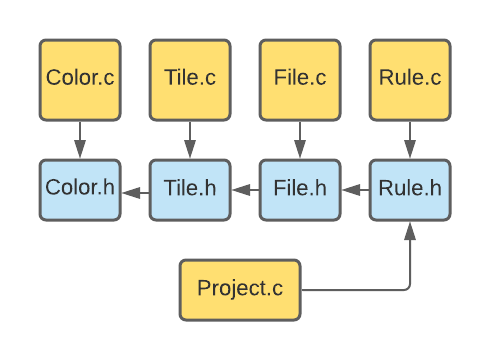
\includegraphics[scale = 0.75]{fichiers1.png}

  \caption{Première interdépendance des fichiers}
  \label{fichier1}
\end{figure}


\subsection{Tests}
Il est essentiel de tester ces fonctions car, si dans certains cas, elles semblent fonctionner, elles pourraient être erronées et nous ne pourrions que difficilement remarquer ces erreurs en lançant le jeu. Ainsi, nous avons décidé de prendre une attention particulière sur les tests. Nous avons divisé les tests en plusieurs fichiers. \\
Le fichier \fbox{test.c} dirige les tests en appelant les fonctions \emph{execute\_test\_{nom\_fichier}}. Cette fonction est définie dans \fbox{test\_{nom\_fichier}.h} et est implémentée dans \fbox{test\_{nom\_fichier}.c}. Elle consiste à appeler les fonctions \emph{test\_{nom\_fonction}}. Ce \emph{{nom\_fichier}} correspond aux fichiers que l'on souhaite tester et \emph{{nom\_fonction}} à ses fonctions. \\
Par exemple, \fbox{test\_color.c} implémente \emph{execute\_test\_color} qui appele \emph{test\_color\_name}. Ainsi, nous avons un système qui centralise les tests de fichiers, eux mêmes découpés en tests de fonctions. \\

Pour cette version initiale, les tests de fonctions se contentent d'afficher 2 cas :
\begin{itemize}
\item Si nous obtenons un résultat différent de celui attendu :  Une erreur est affiché sous la forme ``ERROR: explication de l'erreur''.
\item Si le résultat est équivalent à celui attendu : ``Le \emph{test} est bien \emph{test}''. \\
\end{itemize}

Ce système de test évoluera lors de l'achievement 3 en affichant les erreurs en rouge et les bons résultats en vert. De plus, le nombre d'erreur de chaque fonction et de chaque fichier sera également renvoyé. Ce développement sera expliqué dans la partie ``Ajouts implémentés''. \\


Regardons maintenant les erreurs et problèmes que nous avons pu détectés grâce à nos tests : \\
\begin{itemize}
\item Les tests de \fbox{color.c} n'ont pas posé de problème important si ce n'est d'afficher le \emph{cstring} renvoyé sans changer la couleur dans le terminal. Ce problème a été résolu en copiant le \emph{cstring} retourné, en remplaçant son premier caractère par un ``e'' et en affichant \textbackslash directement dans le \emph{printf} (avant le \%s) plutôt que de simplement appeler le \emph{cstring} dans \emph{printf}.
\item Les tests de \fbox{tile.c} et \fbox{rule.c} se sont confrontés à un problème que nous n'avons pas su résoudre. Pour réaliser ces tests, nous avons besoin de tuiles spécifiques que nous connaissons. Par exemple, pour savoir si un emplacement est valide,  nous devons connaître les couleurs de la tuile en question ainsi que les couleurs celles à proximité. Cependant, la couleur des tuiles dans le deck dépend de \emph{deck\_init}. Nos tests fonctionnent donc avec notre fichier \fbox{tile.c} mais ne peuvent fonctionner avec un autre fichier car les tuiles utilisées seraient différentes et ce changement modifirait donc les résultats attendus. \\
\end{itemize}

Voici un exemple de notre première version des tests :

\begin{figure}[h!]
    \centering
    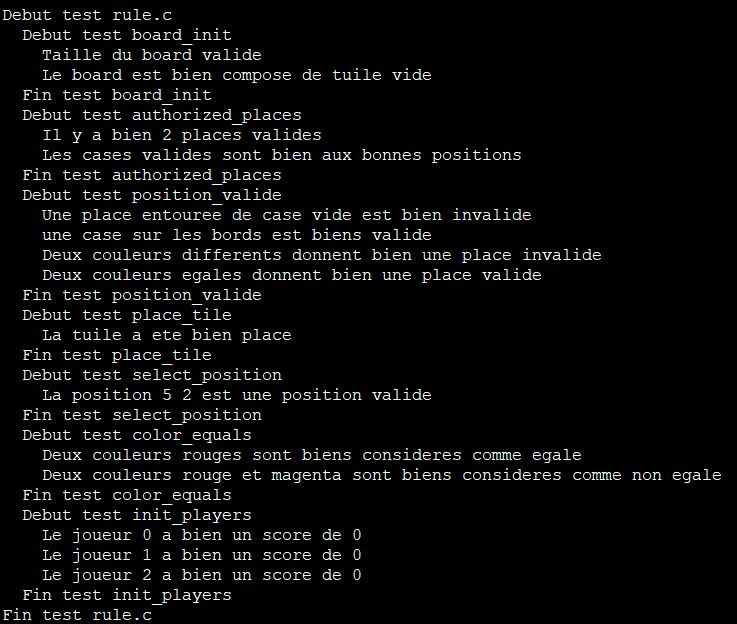
\includegraphics[scale = 0.75]{testV1.jpg}
  
    \caption{Première version des test}
    \label{testV1}
\end{figure}


\section{Apparition de la notion de motifs}
\subsection{Problématiques}
Dans cette nouvelle version du jeu, nous devons maintenant pouvoir implémenter des motifs, une combinaison spécifique de différentes tuiles. Il est également exigé que les méthodes pour construire les motifs soient suffisamment bien écrites pour pouvoir en rajouter aisément. Enfin, on ajoute la notion de propriété car il y a maintenant une importance à savoir quelle tuile appartient à quel joueur. Le calcul des points change également, le score correspond au nombre de motifs réalisé par les tuiles posées par chaque joueur. 

\subsection{Notion propriétaire}
La première modification à faire dans notre jeu initial est d'ajouter un propriétaire pour chaque tuile. Si, précédemment, nous n'en avions pas besoin, car nous ajoutions des points dès qu'un joueur posait une tuile, il est maintenant requis de pouvoir reconnaître le propriétaire de chaque tuile à la fin du jeu. En effet, c'est en récupérant le numéro du joueur qui a posé la tuile centrale que nous pourrons ensuite lui accorder des points via les motifs. \\

Pour ce faire, nous réutilisons la variable \emph{from\_player} de  notre structure \textbf{Board}. Comme son nom l'indique, elle permettra de stocker le numéro du joueur qui pose une tuile à un emplacement (ligne, colonne) et nous permettra de remonter à son propriétaire quand auparavant, cette variable servait uniquement à tester s'il y avait ou non une tuile à ce même emplacement. On initialise cette matrice via la fonction \emph{board\_init} en spécifiant qu'une tuile vide n'a pas de propriétaire et donc prends la valeur -1. 
De cette façon, nous n'avons plus besoin d'appeler la fonction \emph{empty\_tile} pour vérifier si une tuile est vide ou non, il suffit de regarder si la matrice aux mêmes coordonnées possède un propriétaire. Ceci nous permet d'optimiser le programme car il est bien moins coûteux de faire une comparaison à un entier plutôt que de récupérer pour chaque côté la couleur de la tuile et de vérifier si elle est vide ou non. 

\subsection{Gestion des motifs}
Nous souhaitons maintenant définir une structure \textbf{Motif}. Pour cela, nous créons un nouveau fichier (\fbox{motif.h}) qui contient notre définition.
Nous avons besoin pour chaque motif : 
\begin{itemize}
    \item D'une fonction de test qui vérifie si le motif est présent sur le plateau.
    \item D'une variable qui définit si pour cette partie, on décide d'utiliser le motif.
    \item D'une variable score permettant d'évaluer les points relatifs à un motif. \\
\end{itemize}

La principale difficulté dans cette implémentation pour nous fut de définir un pointeur de fonction, car nous ne savions pas comment en créer un. En définitive, il suffit de préciser que c'est un pointeur, de préciser chaque type de variable dont aura besoin la fonction et bien sûr sa valeur de retour. On obtient donc le code ci dessous :

\begin{lstlisting}
struct board;

struct motif
{
    int (* test)(struct board *, int, int);   // Pointeur de fonction
    int actif;
    int score;  
};
\end{lstlisting}

Maintenant que notre structure \textbf{Motif} est définie, il faut une fonction test spécifique à un motif particulier qui puisse le reconnaître sur le plateau. Dans notre jeu, nous avons créé 3 motifs : 
\begin{itemize}
    \item Une tuile entourée de 4 autres tuiles.
    \item Une tuile monochrome à proximité d'au moins deux tuiles bicolores.
    \item Une tuile monochrome à proximité d'au moins une tuile monochrome. \\
\end{itemize}

L'implémentation de ces motifs étant pratiquement similaire, nous n'allons décrire que la fonction test d'une tuile monochrome à proximité d'au moins deux tuiles bicolores.

\begin{enumerate}
    \item \textbf{Fonction is\_monocolor} \\
\newline
Premièrement, on définit une fonction qui prends en paramètre une tuile et qui nous permet de savoir si elle est monochrome ou non. On récupère la couleur d'un côté de la tuile et on compare via la fonction \emph{color\_equals} si elle est égale aux couleurs des 3 autres directions avec l'appel \emph{tile\_edge}. De cette façon, on sait rapidement le type d'une tuile.
\newline
    \item \textbf{Fonction motif\_monocolor\_with\_two\_bicolor} \\
\newline    
Deuxièmement, on crée la fonction qui teste si à un emplacement particulier, une tuile est une tuile centrale dans un motif. Pour cela, la fonction prends en paramètre des coordonnées (ligne, colonne) ainsi que le plateau de jeu. Voici son pseudo-code:

\newpage
\begin{algorithm}
    \caption{Pseudo-code Motif monocolor\_with\_two\_bicolor}
    \begin{algorithmic}
        \IF {N'est pas monocouleur}   
            \RETURN \FALSE
        \ENDIF
        
        \IF {N'est pas sur le bord gauche}
            \STATE On teste si il y a un bicolore à gauche
        \ENDIF
    
        \IF {N'est pas sur le bord droit}
            \STATE On teste si il y a un bicolore à droite
        \ENDIF
        
        \IF {N'est pas sur le bord haut}
            \STATE On teste si il y a un bicolore en haut
        \ENDIF
        
        \IF {N'est pas sur le bord bas}
            \STATE On teste si il y a un bicolore en bas
        \ENDIF
        
        \RETURN ($Bicolore >= 2$)

    \end{algorithmic}
\end{algorithm}

Cette technique nous permet, avec seulement 4 comparaisons, de vérifier si une tuile est sur le bord ou non et elle gère tout les cas. Ces tests sont donc en complexité linéaire O(n) et nous avons préféré une implémentation de ce type plutôt que de traiter les cas où la tuile est sur le bord et de devoir traiter autrement les autres cas. \\

\item \textbf{Appel fonction de test}
Enfin, on souhaite appeler maintenant pour chaque tuile non vide les fonctions de test des motifs. On définit pour cela la fonction \emph{checking\_motif} qui prends en paramètre le nombre de motifs à tester, les joueurs, le plateau et les motifs.
    
\begin{lstlisting}
void checking_motif(struct player players[], struct board *b, int nb_motifs, struct motif motifs[])
{
  for(int i=0; i<(b->taille); i++)
    {
        for(int j=0; j<(b->taille); j++)
	{
          int num = (b->from_player)[i][j];
          if (num != -1)                      //Si la tuile est non vide
	  {
	    for (int m = 0; m < nb_motifs; m ++) 
	    {
              if (motifs[m].actif)        //Si on considère le motif pour cette partie
              {
                if ( (*motifs[m].test)(b,i,j))  //Si la fonction trouve motif est vraie à un emplacement (i, j)
                {
                  players[num].score += motifs[m].score;  
                }
              }
            }
	  }
	}
    }
}
\end{lstlisting}
\end{enumerate}

\newpage

Il reste maintenant à initialiser les motifs dans \fbox{project.c}. Pour cela, nous créons un nouveau motif et nous remplissons ses paramètres en passant la fonction de test de motif en tant qu'adresse. 
Ainsi, nous rajoutons dans l'initialisation :

\begin{lstlisting}
  struct motif m1 = { .score = 3, .actif = 1, .test = &motif_monocolor_with_monocolor };
  struct motif m2 = { .score = 5, .actif = 1, .test = &motif_monocolor_with_two_bicolor };
  struct motif m3 = { .score = 10, .actif = 1, .test = &motif_full_surrond };

  struct motif motifs[3] = {m1, m2, m3};
\end{lstlisting}

De plus, nous souhaitons appeler la vérification des motifs en fin de partie avant d'afficher les résultats. Nous rajoutons donc à la fin de la boucle de jeu l'appel à la fonction de test des motifs comme ceci :

\begin{algorithm}
    \caption{Ajout de l'intégration des motifs à la boucle de jeu}
    \begin{algorithmic}
        \WHILE {Joue}   
            \STATE Le jeu continue comme précédemment 
        \ENDWHILE
    \STATE Vérifie les motifs
    \STATE Affiche les points des joueurs et le vainqueur 
    \end{algorithmic}
\end{algorithm}

Cette implémentation des motifs permet de facilement rajouter des motifs ou d'ajouter un choix des règles où seul certains motifs sont actifs. 
Pour rajouter un motif il suffit : \\ \\
- D'ajouter sa fonction de test dans \fbox{rule.c} et \fbox{rule.h}. \\
- Ensuite, de rajouter dans \fbox{project.c},  \emph{struct motif mX = { .score = {x\_score}, .actif = 1, .test = \&{x\_test} }} avec \emph{{x\_test}} correspondant au nom de la fonction de test que l'on a rajouté et \emph{{x\_score}} au score que nous voulons donner au motif. \\
- Enfin, de changer la valeur du nombre de motif en fonction du nombre de motif rajouté. \\
\newline
Pour le moment, nous avons donc tout les motifs qui sont actifs avec \emph{mX.actif} = 1. Nous avons décidés de rajouter une option -m  <entier> qui permette au joueur de supprimer un ou plusieurs motifs pour la partie. Dès lors que l'on met en argument le motif que l'on souhaite supprimer (numéroté de 1 à 3), le motif n'est plus considéré actif et donc nous n'appelons plus sa fonction test ni n'attribuons de points pour celui-ci.

\subsection{Structure des fichiers}

Pour la gestion des motifs nous avons besoin du fichier \fbox{motif.h} qui contient la définition de la structure \textbf{motif}, \fbox{rule.h} doit donc nécessairement inclure \fbox{motif.h}. La fonction de calcul des scores et les tests des motifs étant dans \fbox{rule.h} il n'est pas nécessaire d'avoir un fichier \fbox{motif.c}. Les autres dépendances n'ont pas évoluées depuis la dernière version.
\newpage

\begin{figure}[h!]
  \centering
  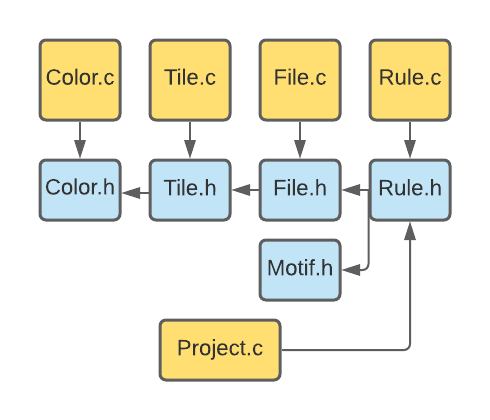
\includegraphics[scale = 0.75]{fichiers2.png}

  \caption{Interdépendance des fichiers}
  \label{fichier2}
\end{figure}


\subsection{Tests}

Les fonctions correspondantes aux motifs ont été uniquement réalisées dans \fbox{rule.c}. Seul le fichier \fbox{test\_rule.c} a changé. Nous avons divisé les tests en 2 fonctions : \\
\begin{itemize}
\item \textbf{La fonction \emph{test\_motifs}}
  Nous créons un plateau avec les 3 motifs et nous vérifions qu'ils sont bien présents avec les bonnes tuiles centrales. Nous vérifions également que sur les autres tuiles, elles ne détectent pas de motifs.
\item \textbf{La fonction \emph{test\_check\_motif}}
  On reprends le même plateau et cette fois, on vérifie que les scores attribués sont égaux aux scores que nous avions calculés pour ce plateau précis. \\
\end{itemize}
On remarquera que ces tests ont également les problèmes précédents car les résultats attendus des tests des motifs dépendent des tuiles utilisées et donc un changement des tuiles définies dans \emph{deck\_init} rend ces tests invalides.

\newpage

\section{Connections des tuiles}
\subsection{Problématiques}
Nous souhaitons maintenant dans cette partie du sujet pouvoir remarquer les connections des couleurs entre les tuiles. Deux tuiles sont connexes si elles possèdent une arête ou un sommet commun. Si on a une connexité, on compte le nombre de tuiles et on attribue au(x) propriétaire(s) ayant le plus de tuiles dans cette zone connexe un score égal au carré du nombre des tuiles de la zone connexe. 

\subsection{Ajout de la connexité}
Rajouter la connexité ressemble à ajouter un motif même si c'est un motif bien plus complexe. En effet, avec la connexité, nous avons de nouvelles difficultés :
\newline
\begin{itemize}
    \item \textbf{Taille variable} \\
Nous ne savons pas quand s'arrête la connexité ce qui complique la recherche du motif. Il faut veiller à ne pas créer de boucles infinies.
    \item \textbf{Pas de tuile centrale} \\
Ici, toutes les tuiles peuvent potentiellement faire gagner des points, ce n'est pas une tuile centrale qui fait remporter tous les points à un seul joueur. Cela implique que tous les joueurs de toutes les tuiles mise en jeu doivent être considérées.
    \item \textbf{On étudie non plus une tuile mais les 4 côtés d'une tuile} \\
Si les motifs étudiaient principalement une tuile dans son ensemble, ici on s'interroge sur les couleurs d'une tuile. Or une tuile possède 4 couleurs ce qui multiplie les tests.
    \item \textbf{Plusieurs gagnants possibles} \\
On peut avoir autant de gagnants sur une connection que de joueurs sur le plateau. Il faut donc s'assurer que tout les gagnants gagnent des points ce qui augmente la complexité. \\
\end{itemize}

Pour répondre à ces difficultés, nous décidons de parcourir chaque tuile à la fin du jeu (à la manière de \emph{checking\_motif}). Pour chaque tuile non vide, nous étudions chacune des couleurs et nous regardons si nous les avons déjà étudié. Si ce n'est pas déjà fait, nous établissons un parcours en profondeur, c'est-à-dire qu'on traverse toute la connexité et on marque chaque couleur traversée comme étant déjà étudiée. \\

On pose la définition ci-dessus en pseudo code :

\begin{algorithm}
    \caption{Pseudo-code de la connexité}
    \begin{algorithmic}
        \FOR {Ligne < taille}
            \FOR {Colonne < taille}
                \FOR {Couleur de tuile < 4 }
                    \IF {Non utilisé \AND Non vide} 
                        \STATE // --  Une couleur ne peut faire partie que d'une seule connexité
                        \STATE Parcourir en profondeur()
                        \STATE Gérer score des gagnants
                    \ENDIF
                \ENDFOR
            \ENDFOR 
        \ENDFOR
    \end{algorithmic}
\end{algorithm}

\begin{algorithm}
    \caption{Pseudo-code du parcours en profondeur}
    \begin{algorithmic}
        \IF {Tuile considérée non étudiée}
            \STATE Tuile considérée comme étudiée à partir de maintenant
        \ENDIF 
        \FOR {Les autres couleurs de la tuile}
            \STATE Appel récursif de parcours\_en\_profondeur
        \ENDFOR
        
        \STATE En fonction du côté proposé
        \STATE On étudie le côté correspondant
        \IF {Côté correspondant n'est pas vide}
            \IF {Couleurs similaires}
                \STATE Appel récursif de parcours\_en\_profondeur
            \ENDIF
        \ENDIF
    \end{algorithmic}
\end{algorithm}

Explications du parcours en profondeur : \\
\begin{enumerate}
\item Nous prenons un côté d'une tuile en argument.
\item La fonction vérifie si les autres côtés de la tuile sont de la même couleur.
\item Enfin, la fonction appelle, pour chaque côté de la même couleur, de manière récursive la fonction \emph{parcours\_en\_profondeur} ce qui permet la diffusion de la connexité. 
\end{enumerate}

Maintenant que nous avons expliqué l'idée de base de ces deux fonctions, nous allons étudier leur implémentation qui est plutôt complexe.

\begin{lstlisting}
  
    void connexe(int nb_player, struct player players[], struct board *b)
    {
        // -- On définit une matrice de tableau
        // ==> Permet d'étudier chaque couleur de chaque tuile du plateau
        /*  * 0 : non traité
            * 1 : déjà traité
            connexe_used[l][c][0] : North
            connexe_used[l][c][1] : South
            connexe_used[l][c][2] : East
            connexe_used[l][c][3] : West
            connexe_used[l][c][4] : Tuile entiere
        */
      int connexe_used[MAX_BOARD_LONG][MAX_BOARD_LONG][5] = {{{0}}};   
      
      for(int l=0; l< b->taille; l++)
        {
            for(int c=0; c< b->taille; c++)
            {
                for(int i=0; i<4; i++)            // Pour chaque couleur
                {
                  if (connexe_used[l][c][i] == 0 && b->from_player[l][c] != -1) {
                    //Initialisation d'une connexité
                struct zone_connexe z = {.nb_tuile = 0, .cases_players = {0}};      
            
/* En effet, si une couleur n'est pas déjà étudié et non vide dans l'appel de connexe
     Alors c'est forcément une connexité non traité que l'on vient de trouvé */
    
                for(int li=0; li< b->taille; li++) {
                    for(int ci=0; ci< b->taille; ci++) {
                  connexe_used[li][ci][4] = 0;
                    }
                }
                
               //On lance le parcours récursif
              parcours_en_profondeur(b, l, c, i, connexe_used, &z);  
     
        // --- On peux considérer à partir d'ici que l'on a terminé l'étude de la connexité
        // On gère maintenant les scores
                
                    int max = 0;
                    int nb_players_max = 0;
                    int players_max[MAX_PLAYERS];
                  
        // --- Sélection des joueurs qui ont le plus de case dans la zone connexe
                    for (int k = 0; k < nb_player; k ++) 
                    {
                        if (max < z.cases_players[k]) 
                        {
                            nb_players_max = 1;
                            players_max[nb_players_max - 1] = k;
                            max = z.cases_players[k];
                        } 
                        else if ( max == z.cases_players[k]) 
                        {
                            nb_players_max ++;
                            players_max[nb_players_max - 1] = k;
                        }
                      }
        
                    // --- Distribution des points
                        for (int v = 0; v < nb_players_max; v ++) 
                        {
                            players[players_max[v]].score += (z.nb_tuile * z.nb_tuile) / nb_players_max; 
                        }
                    }
                }
            }   
        }
    }
    \end{lstlisting}

Cet algorithme s'appuie sur deux éléments qui vont être modifiés et utilisés lors des appels récursif de \emph{parcours\_en\_profondeur} : La structure \textbf{zone\_connexe} et la matrice de tableau \emph{connexe\_used}.
\begin{itemize}
\item  La structure \textbf{zone\_connexe} est utilisée pour l'attribution des scores et possède deux attributs : \emph{nb\_tuile} contient le nombre de tuiles pour le calcul des points et \emph{ cases\_players} est un tableau associant le numéro des joueurs avec le nombre de cases qu'ils possèdent. Lors du troisième achievement, ce sera modifié en la somme des niveaux d'appartenance des cases de la connexité. \\
  
\item La matrice de tableau \emph{connexe\_used} nous permet d'éviter de compter plusieurs fois la même case : \\
  Dans l'appel de la fonction \emph{parcours\_en\_profondeur} à un emplacement (l, c), nous étudions un côté spécifique renseigné par l'entier \emph{i} tel que : 0 (Nord), 1 (Sud), 2(East), 3(West). Si la valeur de \emph{connexe\_used[l][c][i]} est égale à 0, alors nous l'initialisons à 1. Si, en revanche, la valeur est d'ores et déjà à 1, alors le parcours s'arrête car la tuile à déjà été traitée. \\
  
  Ensuite, nous étudions la valeur \emph{connexe\_used[l][c][4]} qui nous permet de déterminer si, pour ce parcours, la tuile a été compté. Si la valeur est égale à 0, alors nous la fixons à 1 et nous incrémentons le nombre de cases totales ainsi que le nombre de cases du propriétaire de la tuile dans la structure \textbf{zone\_connexe}. \\

De cette manière, une case n'est comptée qu'une seule fois dans le même parcours même si plusieurs de ses côtés sont de la même couleur. De plus, une tuile peut être dans plusieurs parcours différents, notamment si elle est composée de plusieurs couleurs. C'est pour cela que dans la fonction \emph{connexe}, entre chaque appel de \emph{parcours\_en\_profondeur}, il faut remettre à 0 \emph{connexe\_used[l][c][4]} en plus de créer une nouvelle structure \textbf{zone\_connexe}. \\
    
Enfin, le parcours va s'appeler sur les autres parties de la tuile si elles sont de même couleur. Pour terminer, le parcours va se propager en fonction du côté opposé de la direction du morceau de tuile qu'il étudie, c'est-à-dire, par exemple, étudier la couleur du côté Sud de la tuile (2, 2) avec l'appel \emph{parcours\_en\_profondeur} du côté Nord de la tuile (3, 2).
\end{itemize}


\subsection{Tests}

Les tests de la connexité sont dans le fichier \fbox{test\_rule.c} car les fonctions \emph{connexe} et \emph{parcours\_en\_profondeur} sont dans \fbox{rule.c}. Ces tests sont regroupés dans la fonction \emph{test\_zonne\_connexe} qui va créer un plateau puis appeler les fonctions \emph{test\_parcours\_en\_profondeur}et \emph{test\_connexe}, qui testent respectivement \emph{parcours\_en\_profondeur} et \emph{connexe}, en leur donnant un plateau spécifique. Ces tests, se basant sur les couleurs des tuiles, seraient obsolètes au moindre changement de tuile dans le deck et un deck de moins de 5 tuiles provoquerais une erreur de segmentation car pour créer le tableau nous utilisons la 5ème tuile.  

\section{Influence des joueurs sur les tuiles}
\subsection{Problématiques}
\begin{itemize}
    \item Premièrement, nous souhaiton maintenant que les tuiles puissent changer de propriétaire. Pour cela, le programme attribue à chaque tuile un niveau d'influence pour chacun des joueurs. A chaque fois qu'un joueur joue une tuile, ce joueur la possède par une influence de 100, tous les autres n'ont aucune influence sur la tuile. Puis, à chaque tuile posée à côté de cette même tuile, le programme attribue une certaine influence en fonction des tuiles déjà pré-disposées. Enfin, à chaque fin de tour, une fonction réduit l'influence de tout les joueurs de 1 pour chacune des tuiles. \\
    
    \item Deuxièmement, nous souhaiton maintenant implémenter une mécanique aléatoire, Le King, qui choisit une case du plateau et en cas de découverte d'une tuile, réduirait l'influence du (des) propriétaire(s) de 50 sur la tuile et toutes les autres tuiles connexes sur une même ligne ou une même colonne que la tuile ciblée. \\
    
    \item Troisièmement, le(s) propriétaire(s) d'une connexité corresponde(nt) maintenant au(x) joueur(s) dont la somme des influences de toutes les tuiles de la zone connexe est maximale.
\end{itemize}

\subsection{Implémentation de l'influence}

L'influence permet de déterminer le(s) propriétaire(s) d'une case nous avons donc décider de modifié \emph{from\_player} du plateau pour l'implémenter. Il transforme la matrice \emph{from\_player[ligne][colonne]} en une matrice de tableau \emph{from\_player[ligne][colonne][numéro\_joueur]}. Les noms \emph{ligne} et \emph{colonne} correspondent toujours à un emplacement (ligne, colonne) et \emph{numéro\_joueur} correspond au numéro du joueur. Ainsi, \emph{from\_player[l][c][numéro\_joueur]} donne désormais le niveau d'appartenance du joueur \emph{players[numéro\_joueur]} sur la tuile en position (ligne, colonne). \\
\\
L'implémentation de la réduction d'influence, nommée \emph{update\_propriete} défini dans \fbox{rule.c}, est donc triviale car il suffit d'une boucle sur toutes les lignes, les colonnes et les numéros des joueurs en vérifiant si l'influence des joueurs est supérieur à 0. Si c'est le cas, nous la réduisons de 1. Cependant, cela cause des problèmes avec nos précédentes utilisations de \emph{from\_player}.

\subsection{Conséquences sur les fonctions existantes}

L'initialisation de \emph{from\_player} change pour correspondre à sa nouvelle définition. Cependant le principe reste le même et lors de l'initalisation de plateau on met la valeur à -1 pour tous les numéros de joueurs sur toutes les lignes et les colonnes.\\
\\

Une des premières utilisations modifiées immédiatement est notre test de case vide en comparant \emph{from\_player[ligne][colonne]} avec -1. Le nombre de joueurs est variable, mais il y a toujours au moins un joueur. Sachant que l'influence est initialisé à -1, que dès qu'une tuile est placée, un des joueurs à une influence de 100 et tout les autres ont une influence égale à 0 et que l'influence des joueurs sur une tuile ne peut descendre en dessous de 0,  il suffit donc de comparer \emph{from\_player[ligne][colonne][0]} avec -1 pour déterminer si la case est vide ou non. Nous pouvons garder ce fonctionnement avec cette simple mise à jour.\\
\\
Le placement d'une tuile change de 2 façons : \\
\begin{itemize}
  \item En premier lieu, plutôt que d'avoir seulement le numéro du joueur qui place une tuile, il faut initialisé l'influence à 100 pour ce joueur sur cette tuile et 0 pour le reste d'entre eux. C'est trivial, une boucle met l'inflluence de tout le monde à 0 puis on met à 100 la valeur \emph{from\_player[numéro du joueur qui la placée]} (donné en paramètre de la fonction). \\
  \item Deuxièmement, il faut maintenant implémenté l'ajout de l'influence sur les cases à côté en fonction du nombre de cases placées avant, ce qui est plus complexe. Nous avions d'abord décidé de compter le nombre de case non vide à côté de la case dont on doit modifier l'influence mais nous avons finalement décidé, pour réduire le nombre de tests, de rajouter l'attribut \emph{nb\_tuiles\_placed\_after}, initialisé à 0, dans la structure \textbf{Board}. Ainsi, il nous suffit donc d'augmenter cette valeur de 1 et d'ajouter à l'influence (100 - 10 * \emph{nb\_tuiles\_placed\_after[l][c]}) pour le joueur posant la tuile à proximité. \\
\end{itemize}

Les points pour un motif sont attribués au(x) propriétaire(s) de la tuile centrale du motif. Désormais, il peut y avoir plusieurs propriétaires dès lors que la tuile centrale à plusieurs joueurs avec un même niveau maximum d'influence. Nous avons donc décider de créer une fonction \emph{proprietaires} qui prends en paramètre le plateau (b), une ligne (l), une colonne (c), le nombre de joueurs dans la partie \emph{(nb\_players)} et d'un tableau d'une taille supérieur ou égale à \emph{nb\_players} \emph{(proprios)}. Elle remplis le tableau \emph{proprios} avec les numéros des joueurs qui ont la valeur d'influence la plus grande pour la tuile en position (l, c) et retourne leur nombre. Grâce à cette fonction, il suffit de l'utiliser sur la tuile centrale d'un motif puis de faire une boucle sur les éléments de \emph{proprios} de 0 au nombre retourné par \emph{proprietaires}. Dans la boucle, nous aurons donc les numéros des joueurs pour lesquels il faut augmenter le score.\\

Pour les zones connexes, \emph{cases\_players} correspond désormais à la somme de l'influence de chaque case de la zone pour le joueur. Il suffit donc de changer, dans le \emph{parcours\_en\_profondeur}, l'incrémentation de cette valeur en une somme de l'influence des joueurs d'une tuile de la connexité et de l'influence des joueurs des autres tuiles. Le programme stocke au fur et à mesure cette influence ttale dans \emph{cases\_players[numero\_joueur]}. Le reste du comportement ne diffère pas. \\


\subsection{Implémentation du King}
Nous pouvons résumer l'action du King par une unique fonction que l'on crée dans \fbox{rule.c} car plutôt que de voir le King comme étant un joueur spécial, on peut considérer que c'est simplement une nouvelle règle dans le jeu. Elle prends plusieurs paramètres : Le plateau, le nombre de joueurs mais également un emplacement (ligne, colonne) aléatoire. Voici son pseudo-code :
\newpage

\begin{algorithm}
    \caption{Pseudo-code du King}
    \begin{algorithmic}
        \IF {A l'emplacement (l, c) il y a une tuile}
            \STATE P = le(s) propriétaire(s)
            \IF {$P.Influence >= 50$}
                \STATE P.Influence -= 50
            \ELSE
                \STATE P.Influence = 0
            \ENDIF
        \ENDIF
        
        \STATE // - Etude connexité
        \STATE      // --- Ligne
        \WHILE {Pas sur le bord gauche}
            \STATE Décalage vers la gauche
            \STATE P = le(s) propriétaire(s)
            \IF {$P.Influence >= 50$}
                \STATE P.Influence -= 50
            \ELSE
                \STATE P.Influence = 0
            \ENDIF
        \ENDWHILE
        
        \WHILE {Pas sur le bord droit}
            \STATE Décalage vers la droite
            \STATE On récupère le(s) propriétaire(s)
            \IF {$P.Influence >= 50$}
                \STATE P.Influence -= 50
            \ELSE
                \STATE P.Influence = 0
            \ENDIF
        \ENDWHILE
        
        \STATE      // --- Colonne
        \STATE          ...
        
    \end{algorithmic}
\end{algorithm}

\subsection{Appel des fonctions dans la boucle de jeu}
Dès lors, il suffit d'appeler les nouvelles fonctions à chaque fin de tour dans la boucle de jeu :

\begin{lstlisting}
    //Fin d'un tour
    if (active_player == (nb_players - 1))
      {
    	update_propriete(&b, nb_players);
    	
    	int chosed_l = rand() % b.taille;
    	int chosed_c = rand() % b.taille;
    	active_player = 0;
    	king(&b, nb_players, chosed_l, chosed_c);
      }
\end{lstlisting}

\subsection{Tests}

De la même façon que les fonctions pour la connexité, les fonctions gérant l'influence sont également dans \fbox{rule.c}. Les tests de l'influence sont donc égalements dans \fbox{test\_rule.c}. Ces tests correspondent à une mise a jour des tests des fonctions modifiées (\emph{place\_tile}, \emph{motifs}, ...) et des nouvelles fonctions (\emph{king} et \emph{update\_propriete}). Ces fonctions, ne dépendant pas des couleurs, permettent aux tests de rester valide lors d'un changement de deck à condition que le deck contient toujours au moins 5 tuiles différentes car la 5ème tuile du deck est utilisée pour construire la structure \textbf{Board}.


\section{Conclusion}

\subsection{Ajouts implémentés}
En plus des consignes apportés par les différents achievments, nous avons implémentés des fonctions/outils supplémentaires pour les joueurs. Si une partie de ces modifications a déjà été expliqué, nous préférons tout de même les réécrire ici pour centraliser ces ajouts : \\

\begin{itemize}
    \item \textbf{Amélioration des tests.}\\ Pendant une grande partie du projet, les tests s'affichait avec la couleur classique du terminal et affichait uniquement un message si tout fonctionnait correspond ou s'il y avait une erreur. Pour facilité la lecture, nous avons décidé d'afficher les erreurs en rouge, d'afficher les résultats attendus en vert et d'afficher le nombre d'erreurs total, par fichier et par fonction. Les fonctions de test ne sont alors plus des \emph{void} mais des \emph{int} et elles renvoient le nombre d'erreur trouvé. Pour cela nous avons créé deux fichiers outils.c et outils.h qui regroupent des fonctions utilent pour les tests : les changements de couleurs (rouge/vert/blanc) et un \emph{template} pour afficher le nombre d'erreurs.\\
    \begin{figure}[h!]
        \centering
        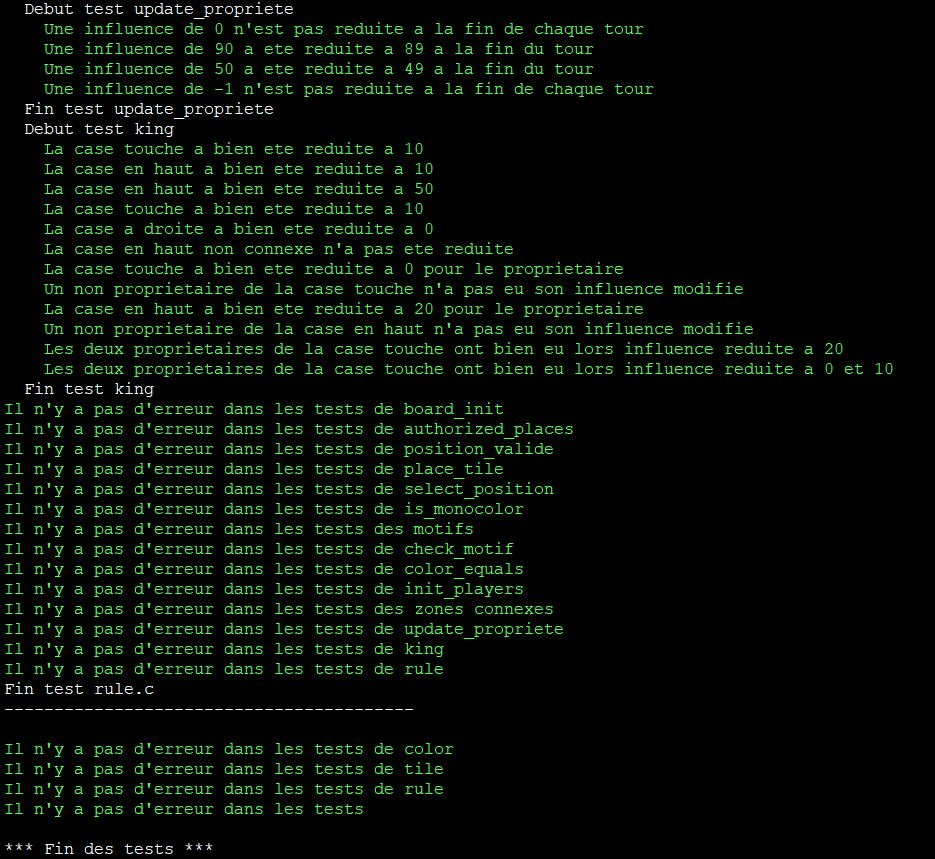
\includegraphics[scale = 0.75]{testV2.jpg}
      
        \caption{Version finale des test}
        \label{testV2}
    \end{figure}
    \newpage
    
  \item \textbf{Rendu visuel plateau via l'option -r } \\
Affiche le plateau avec les bords des tuiles en couleurs, avec à l'intérieur le numéro du propriétaire s'il y en a un unique "pl" sinon et l'influence du propriétaire si elle est inférieure à 100 ou "C+" dans le cas contraire. \\
    
    \begin{figure}[h!]
        \centering
        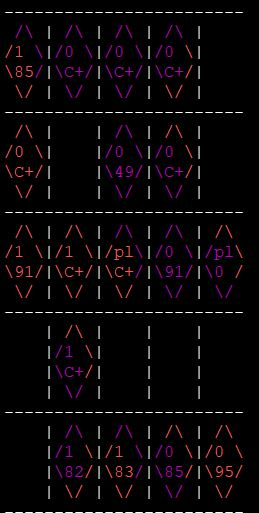
\includegraphics[scale = 0.75]{board.jpg}
      
        \caption{Plateau de jeu}
        \label{board}
    \end{figure}

    \item \textbf{Supprimer des motifs via l'option -m} \\
En plus de pouvoir créer des motifs de façon générique, nous avons implémenté en bonus une option -m <entier> permettant de supprimer des règles du jeu un motif pour une partie. De cette façon, on peut à la fois rajouter facilement et supprimer facilement des motifs d'une partie. \\
    
  \item \textbf{Rendu visuel influence via l'option -i } \\
    Affiche pour chaque tuile l'influence de chaque joueur.

    \newpage
    
    \begin{figure}[h!]
        \centering
        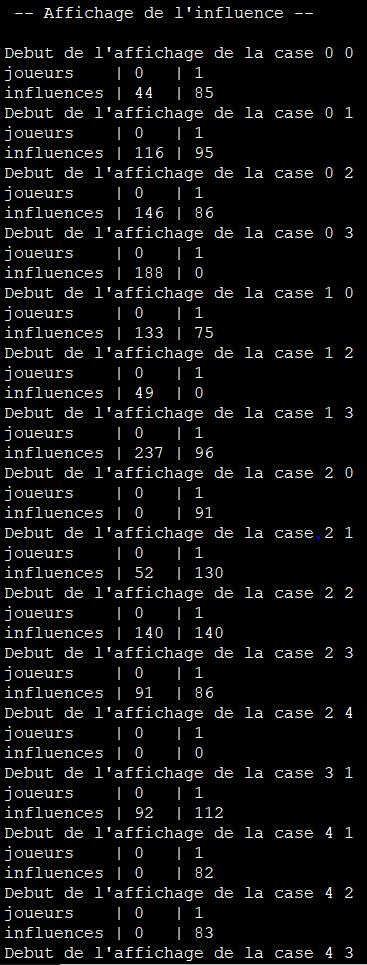
\includegraphics[scale = 0.75]{influence.jpg}
      
        \caption{L'influence des joueurs}
        \label{influence}
    \end{figure}

      
     \item \textbf{Limiter la casse au niveau des options} \\
Qu'advient-il si nous décidons de jouer une partie avec un nombre de joueurs négatifs ? Ou un seul joueur ? De la même façon, que renvois notre programme si l'on lance une partie avec un plateau de taille négative ? Pour gérer ces cas "extrêmes", nous définissons des variables par défaut dans \fbox{rule.h} :

\begin{lstlisting}
#define MAX_PLAYERS 20
#define MAX_BOARD_LONG 50
#define DEFAULT_BOARD_LONG 10
\end{lstlisting}

De cette façon, tous les problèmes sont résolus : \\
Si les joueurs tentent de jouer sur un plateau trop grand, d'appeler un nombre négatif de joueurs, etc, alors le système prends des paramètres par défaut c'est-à-dire 20 pour le nombre de joueurs et 10 pour la taille du plateau. \\ \\

De plus, si le joueur met de mauvais arguments, par exemple "-v", alors le programme lui affiche comment l'utiliser :

\begin{lstlisting}
./project: invalid option -- 'v'
Usage: ./project [-s seed] 
Usage: ./project [-n number of players] 
Usage: ./project [-b width of the board] 
Usage: ./project [-r] Print results 
Usage: ./project [-i] Print influence
Usage: ./project [-m which motif retired] 
\end{lstlisting}

Ainsi, si l'utilisateur n'a pas lu le fichier \fbox{README.txt}, il peut quand même comprendre le fonctionnement du programme.

\end{itemize}



\subsection{Ce que nous a apporté le projet}
Ce projet nous a permis de développer des compétences techniques. Nous avons progressé dans notre maîtrise du langage C et du makefile lors du développement, dans notre connaissance de LaTeX pour l'écriture de ce rapport et dans notre utilisation de Git durant toute la durée du projet. Nous avons également appris à travailler en équipe, comment réfléchir ensemble aux problèmes posés par le sujet, avant de se répartir les tâches pour l'implémentation des solutions. Nous sommes très satisfait de ce projet et avons beaucoup apprécié notre collaboration en tant que binôme.


\end{document}
